%!TEX root = ../NCVC.tex

\mysection{応用編}

\subsection{方向制御}
 結論から言うと,普通の方法では方向制御できません.
例えば1つの座標に複数のオブジェクトが接続されている場合,NCVCが最初にどれを選択するかは内部で独自に決定されます.
ここでは応用編の第一弾としてムリヤリ(?)方向制御を行う方法を解説します.

\begin{minipage}[t]{0.5\textwidth}
 図\ref{fig:direction}を見てください.
中心の加工原点と左下の加工開始を示す円データ,五角形の線データがあります(それ以外は補助線).
一見して普通の作図,\ref{sec:move}節で解説した移動レイヤだけに見えますが,実は複数レイヤ処理との合わせ技で作図されています.
図\ref{fig:direction.png} は図\ref{fig:direction}のCADデータを読み込み,レイヤ表示で切削レイヤの2つ目を非表示にした状態を表しています.
\end{minipage}
\begin{minipage}[t]{0.5\textwidth}
\vspace*{-2zh}
\begin{figure}[H]
\centering
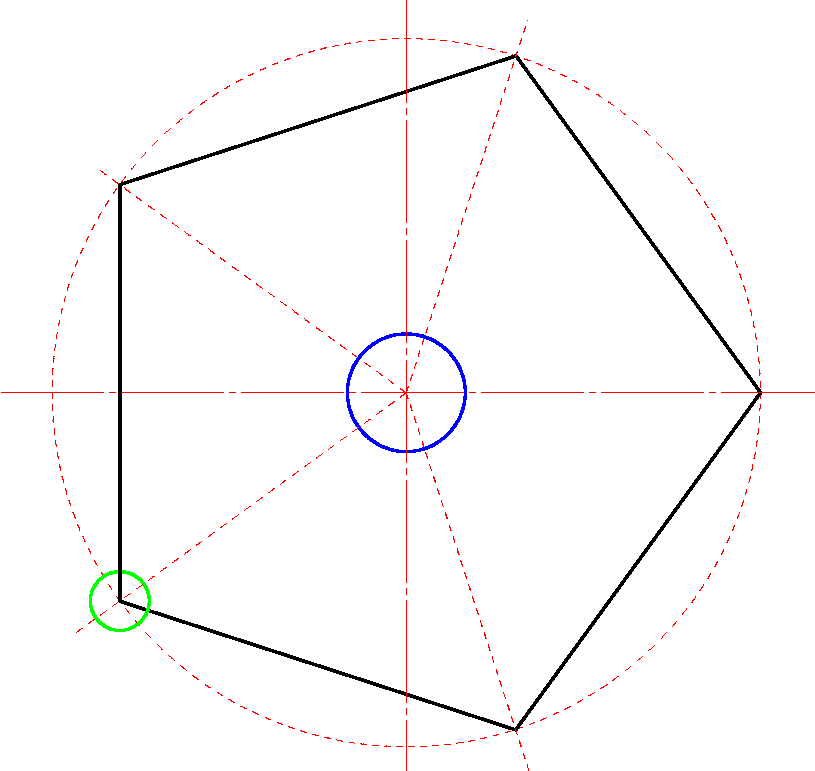
\includegraphics[width=\textwidth]{No4/fig/direction-crop.pdf}
\caption{方向制御作図例}
\label{fig:direction}
\end{figure}
\end{minipage}

\begin{figure}[H]
\centering
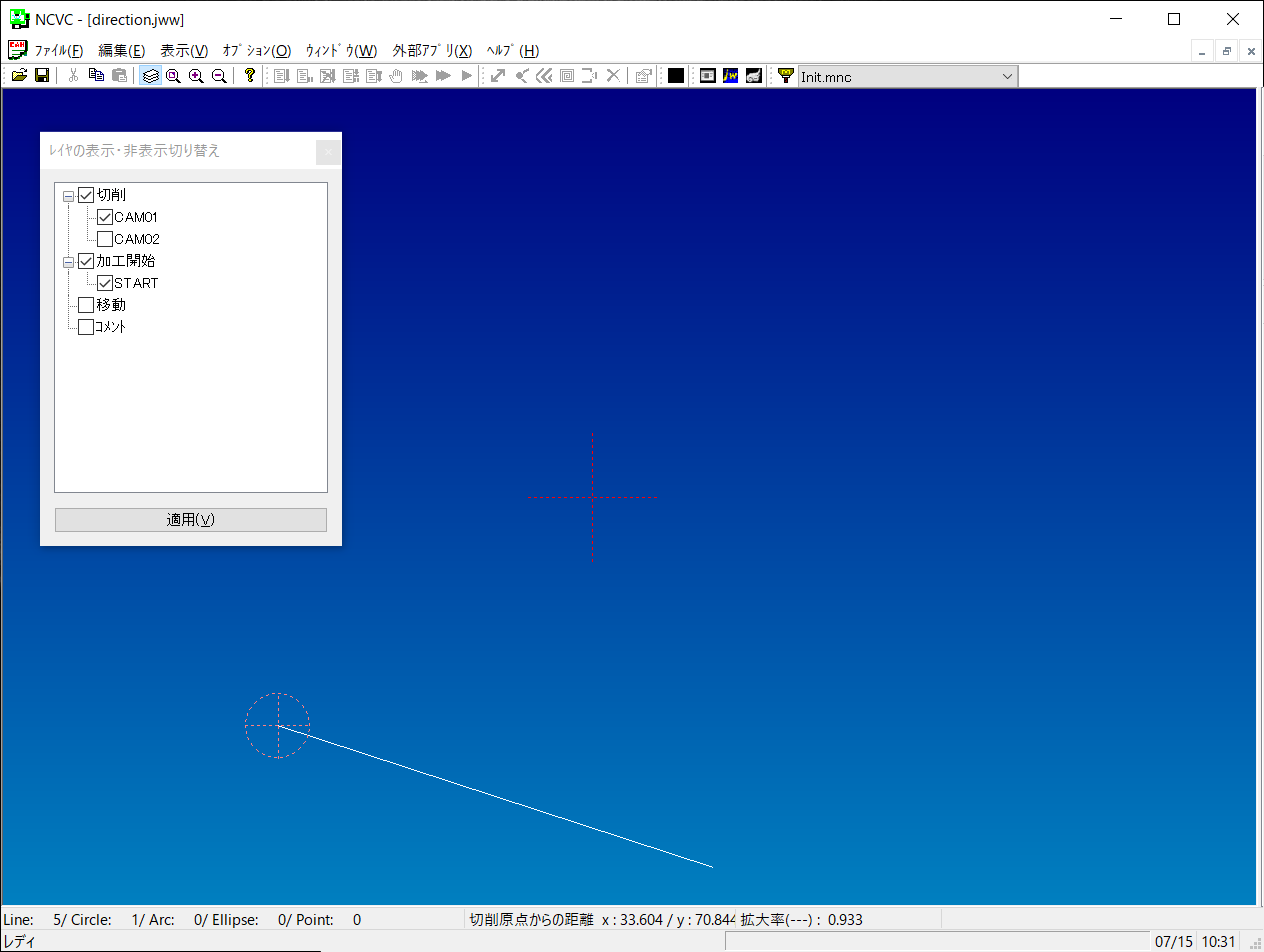
\includegraphics[scale=0.55]{No4/fig/direction.png}
\caption{複数レイヤを読み込んだ状態}
\label{fig:direction.png}
\end{figure}

\begin{minipage}[t]{0.5\textwidth}
 もうお解りですね.開始したい座標に複数のオブジェクトがあれば,それを違うレイヤに作図し,方向が明確に示せるようにすればOKです.
ただし,複数レイヤ処理を行う必要があるので,単一条件でのNC生成では希望通り生成できません.
【\ref{sec:multi-layer} 複数レイヤ処理】で解説した拡張NC生成,[レイヤごとのZ座標指定]か[レイヤごとの切削条件]で処理する必要があります.
どちらの場合でも同じZ値,または,同じ条件を割り当てることができます(図\ref{fig:direction-setup}).
\end{minipage}
\begin{minipage}[t]{0.5\textwidth}
\vspace*{-2zh}
\begin{figure}[H]
\centering
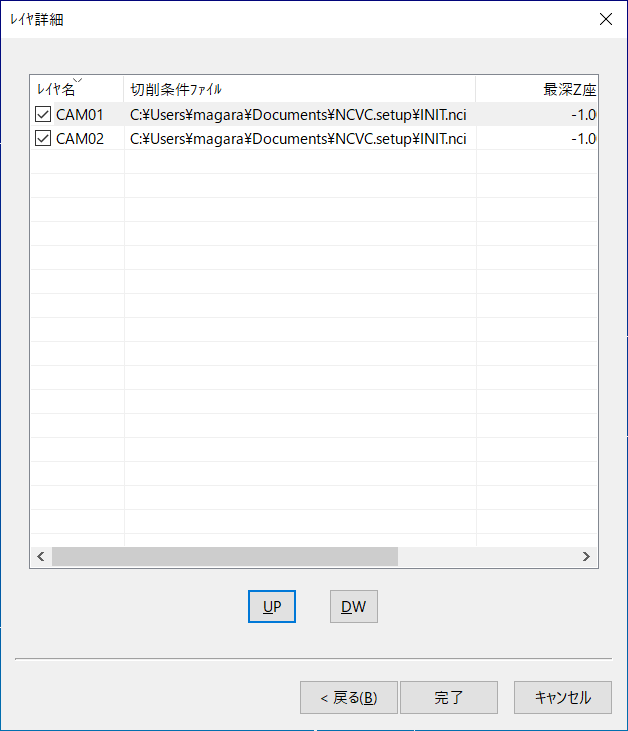
\includegraphics[scale=0.6]{No4/fig/direction-setup.png}
\caption{2つの切削レイヤに同じ加工条件を割り当て}
\label{fig:direction-setup}
\end{figure}
\end{minipage}

\vspace*{2zh}
\begin{minipage}[t]{0.6\textwidth}
 もう1つ,裏技的というより,これぞムリヤリですが(自爆)要するに1つの座標に2つ以上のオブジェクトを作図しなければ良いだけで,
例えば図\ref{fig:direction2} のように矩形切削の方向を指示したい場合,影響の無い範囲内で他方の座標をずらしてやれば良いのです.
前の切削領域からの最短距離ならNCVCが自動で検索します.明確に指示したい場合は【\ref{sec:move} 移動レイヤ】が使えます.
\end{minipage}
\begin{minipage}[t]{0.4\textwidth}
\vspace*{-2zh}
\begin{figure}[H]
\centering
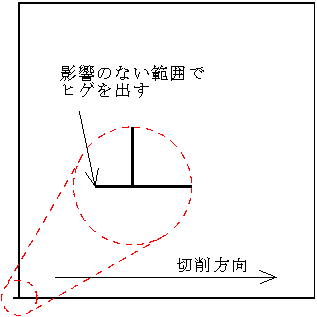
\includegraphics[width=\textwidth]{No4/fig/direction2-crop.pdf}
\caption{矩形切削例}
\label{fig:direction2}
\end{figure}
\end{minipage}

\vspace*{2zh}
 どちらにしてもあまり格好の良い方法ではありませんね...

\subsection{形状切削}
 方向制御と同じく形状切削についてもNCVCでは生成できません.
一般的にCADでは完成された形状を作図しますが,実際の加工では工具の半径を考慮しなければなりません.
特に島加工・ポケット加工については,CADで作図した形状情報からNCVCが加工データを生成できません.
NCVCはCADのデータを工具の軌跡データと扱うのです.

 もうカンの良い皆様ならお気づきだと思います.
NCVCで形状切削の加工データを得るには,今度こそCADの力を存分に借りる必要があります.
図\ref{fig:keijyou} は【\ref{sec:hole} 穴加工】のサンプルデータ(p.\pageref{fig:sample2.pdf})からポケット加工のデータを得るための作図例です.
工具半径や必要な肉厚を考慮しつつCADの複線機能を駆使して作図しました.
面倒そうですが慣れると意外と簡単に作図できます\footnote{ご使用のCADの性能や習熟度次第ですが...}.
削りすぎにはくれぐれもご注意を(体験談).
削り残しも作図段階でチェックできませんが
\footnote{Jw\_cad の場合,円の作図で半径を入力すれば,これから作図しようとする円が表示されます.
これを工具に見立ててマウスを動かせば簡易チェッカ(?).無論補助レイヤにて工具円を書きまくるのが確実デス.},
NCVCのシミュレーション画面もワイヤー表示なので,どのみちチェックできませんね(自爆x2)

\begin{figure}[H]
\centering
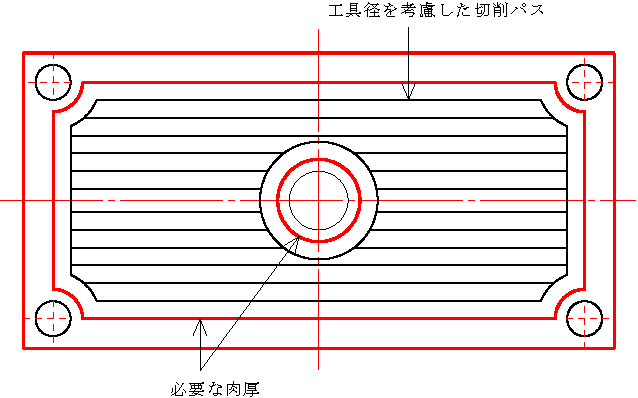
\includegraphics{No4/fig/keijyou-crop.pdf}
\caption{ポケット加工作図例}
\label{fig:keijyou.pdf}
\end{figure}

\vspace*{2zh}
\begin{itembox}[l]{ここまでの【まとめ】}
\begin{itemize}
\item 方向制御と形状切削は,CADの作図次第
\item スマートに指示するにはもう少しNCVCの進化を待つ必要がある
\end{itemize}
\end{itembox}
